\documentclass[ngerman,aspectratio=169,10pt]{beamer}

\usetheme[progressbar=frametitle]{metropolis}
\usepackage{appendixnumberbeamer}

\graphicspath{{./graphics/}, {./../../data/scripts/runs/rules/figures/}, {./../../data/scripts/runs/simulAn/figures/}}

\usepackage{booktabs}
\usepackage{xspace}
\usepackage{amsmath}
\usepackage{amssymb}
\usepackage{amsthm}
\usepackage{xfrac}
\usepackage{listings}
\lstset{
	basicstyle=\ttfamily,
	showstringspaces=false,
	tabsize=4,
	upquote=true,
}

\title{Labeling-Heuristiken}
% \subtitle{}
\date{09. Dezember 2020}
\author{Levin Nemesch, Joshua Sangmeister}
\institute{Algorithm Engineering - Projekt}
\titlegraphic{
    \hfill
\includegraphics[height=1.5cm]{unilogo.pdf}\\
    \hspace*{8.3cm} \textsc{AG Theoretische Informatik}
}

\begin{document}

\maketitle



\begin{frame}{Rules-Heuristik: Definitionen}
    \begin{itemize}
        % @Levin: Falls du die Definitionen auch nutzen willst/brauchst, schieb sie gerne nach oben und schmeiß diese Folie einfach raus, die 2 Phasen kann ich auch mündlich sagen
        % @Joshua: Ok, kann ich tatsächlich gebrauchen
        \item Ein \textit{Punkt} hat mehrere \textit{Kandidaten}
        \item Kandidaten können \textit{in Konflikt stehen}
        \item Die \textit{Konflikt-Partner} eines Kandidaten sind alle Kandidaten, mit denen er in Konflikt steht
        \item \textit{Konfliktzahl} eines Kandidaten: Anzahl der Konflikt-Partner
    \end{itemize}
\end{frame}


\begin{frame}{Conflict Array}
    \begin{itemize}
        \item Speichert für jedes Label alle möglichen Konflikt Partner
        \item Erlaubt später schnelleres Prüfen ob ein Label ein anderes Überlappt
        \item Aber: Keine Garantie für Größe, möglicherweise kollidieren alle Label
        \item Alternative: Segment trees
        \item Conflict arrays können cache locality ausnutzen
    \end{itemize}
\end{frame}


\begin{frame}[fragile]{Referenzheuristik}
    \begin{itemize} 
        \item Erzeugt gute Lösung in $O(n^2) \longrightarrow$ Benchmark für Heuristik
        \item Algorithmus:
    \end{itemize}

    \begin{lstlisting}
    set all labels false 
    for all labels in order:
        for every candidate in random order:
            if no conflict for position:
                set label to position
                break
    \end{lstlisting}
\end{frame}

\begin{frame}{Simulated Annealing: Konzept}
    \begin{itemize} 
    \item Ähnlich wie Gradientenabstieg, erlaubt aber temporäre Verschlechterung
    \item Simuliert sinkende Energie in sich stabilisiernden System
    \item Zielfunktion E
    \item Verbesserungen von E werden immer akzeptiert
    \item Verschlechterungen von E werden mit über Zeit sinkender Wkt akzeptiert
    \end{itemize} 
\end{frame}

\begin{frame}[fragile]{Simulated Annealing: Algorithmus}
    % Diese Folie werde ich in der Präsi nur anreißen, sie ist der Vollständigkeit halber aber drinnen
    \begin{lstlisting}
        while temperature above threshold:
            for number_of_tries:
                change label
                if new E lower than previous E:
                    decide if to keep solution
                else:
                    keep solution
            lower temperature
        \end{lstlisting}
\end{frame}

\begin{frame}[fragile]{Simulated Annealing: Try New Label}
    \begin{enumerate} 
    \item Wähle zufälliges Label L
    \item Setzte L auf zufällige und neue Position
    \item Finde kollidierende Label und verschiebe oder entferne diese
    \item Falls E verschlechtert: Behalte mit $P=1-\exp^{-\frac{\Delta E}{t}}$
    \end{enumerate} 
\end{frame}

\begin{frame}[fragile]{Simulated Annealing:Feste Faktoren}
    \begin{itemize} 
    \item E: Anzahl aktiver Label
    \item Abkühlungsrate: $0.9$
    \item Zusätzlicher Abbruch, falls bereits Hälfte aller erlaubten Werte verändert\\
    (Annahme, dass Energie in diesem Fall viel zu hoch)
    \end{itemize} 
\end{frame}

\begin{frame}{Simulated Annealing: Variable Faktoren}
    \begin{itemize} 
    \item Starttemperatur ($\log(n)$, $\sqrt(n)$, $\frac{\sqrt(n)}{3}$, $\sqrt(n)*\log(n)$, $n$)
    \item Versuche pro Temperatur (1, 2, 4, 8)
    \item Label nicht initialisiert oder mit Referenzheuristik
    \end{itemize} 
    (Getestete Werte in Klammern)
\end{frame}

\begin{frame}{Simulated Annealing: Parametervariation}
    \begin{itemize} 
    \item Auf kleinen Instanzen macht sich Variation kaum bemerkbar
    \item Auf großen Instanzen Initialisierung nötig
    \item Höhere Temperatur kaum Verbesserung $\rightarrow t=1$
    \item Je mehr Versuche pro Temperatur, desto besser Ergebnis\\
    $\Longrightarrow$ Wurzel zu klein, linear zu groß $\rightarrow \sqrt(n)*\log(n)$ guter Kompromiss
    
    \end{itemize} 
\end{frame}

\begin{frame}{Simulated Annealing: Lösungsgüte I}
    \centering
    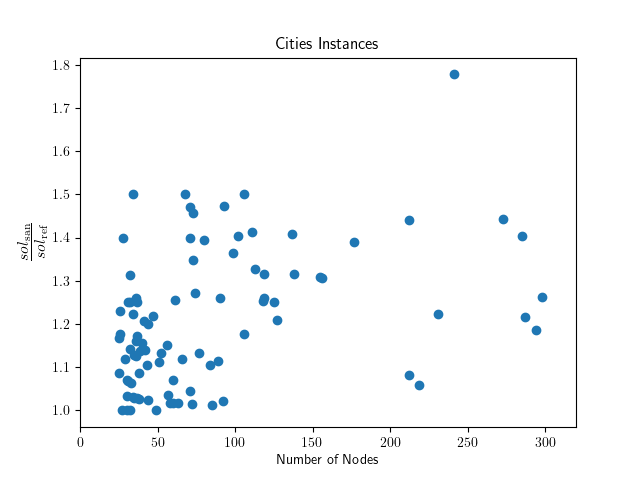
\includegraphics[width=270px]{countries_labs}
\end{frame}

\begin{frame}{Simulated Annealing: Lösungsgüte II}
    \centering
    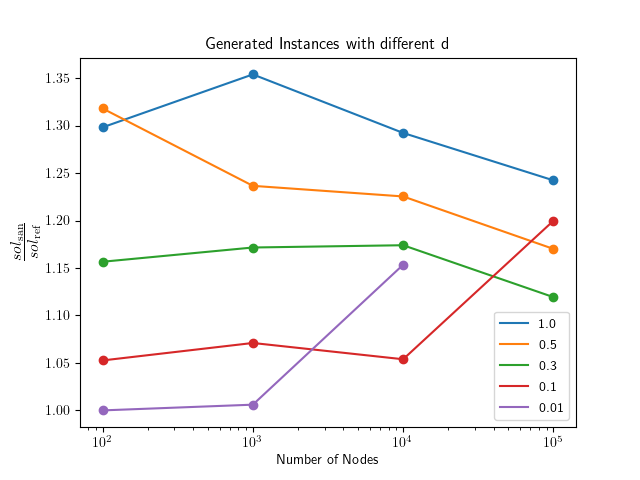
\includegraphics[width=270px]{generated_labs}
\end{frame}

\begin{frame}{Simulated Annealing: Zeitaufwand Relativ I}
    \centering
    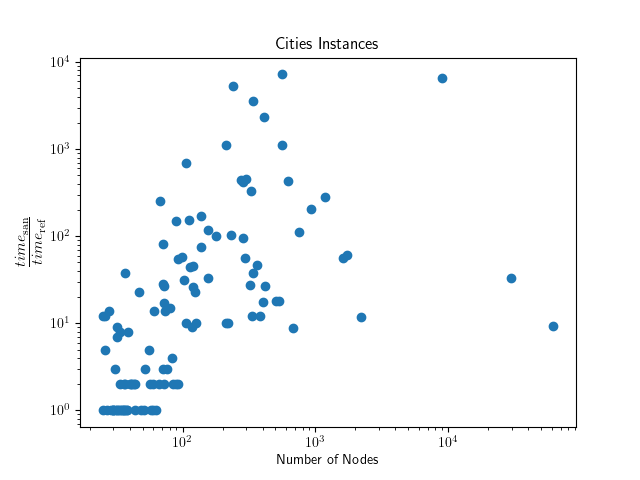
\includegraphics[width=270px]{countries_time_rel}
\end{frame}

\begin{frame}{Simulated Annealing: Zeitaufwand Absolut I}
    \centering
    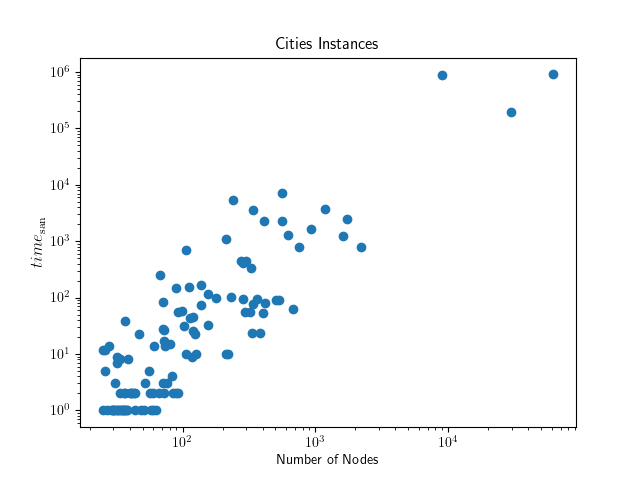
\includegraphics[width=270px]{countries_time_abs}
\end{frame}

\begin{frame}{Simulated Annealing: Zeitaufwand Relativ II}
    \centering
    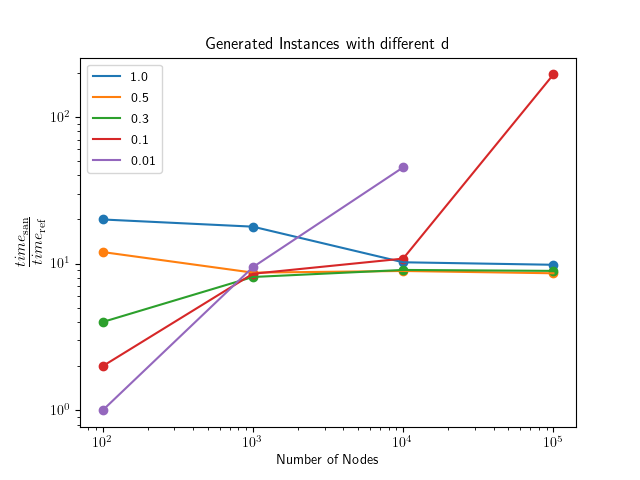
\includegraphics[width=270px]{generated_time_rel}
\end{frame}

\begin{frame}{Simulated Annealing: Zeitaufwand Absolut II}
    \centering
    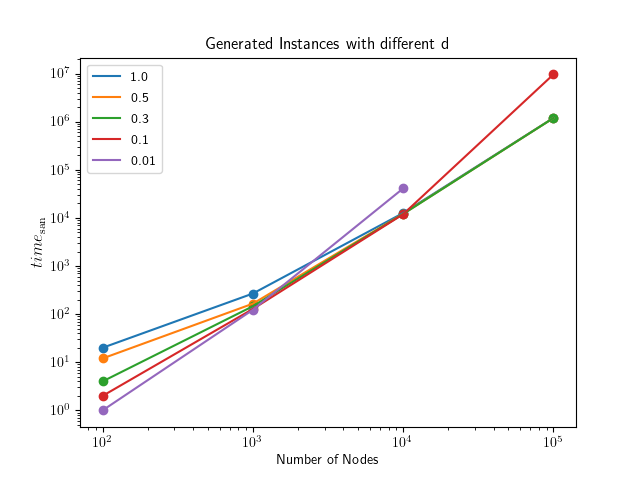
\includegraphics[width=270px]{generated_time_abs}
\end{frame}

\begin{frame}{Weitere Arbeit}
    \begin{itemize}
        \item Bestes im Algorithmus erreichter Wert immer Endwert\\
        $\Longrightarrow$ Ist wie Gradientenabstieg?
        \item Kein Implementationsfehler, einzelne Verschlechterungen kommen vor\\
        $\Longrightarrow$ Energie nicht ausreichend um Bereich des lok. Mins zu verlassen
        \item Parameteraum für höhere Energiewerte absuchen
        \item Abkühlungsrate in Relation zu initialer Energie setzen
        \item Zeitlimit
    \end{itemize}
\end{frame}

\begin{frame}{Rules-Heuristik}
    \centering
    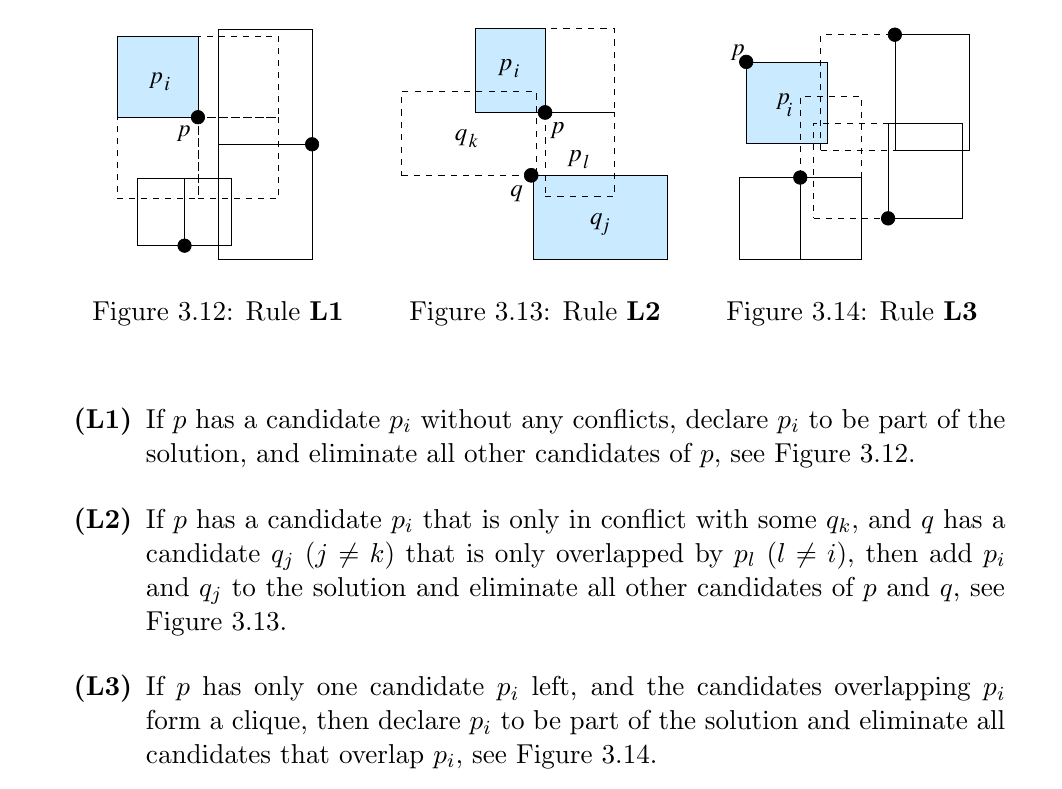
\includegraphics[width=270px]{rules}
\end{frame}

\begin{frame}{Rules-Heuristik: Ergebnisse}
    \centering
    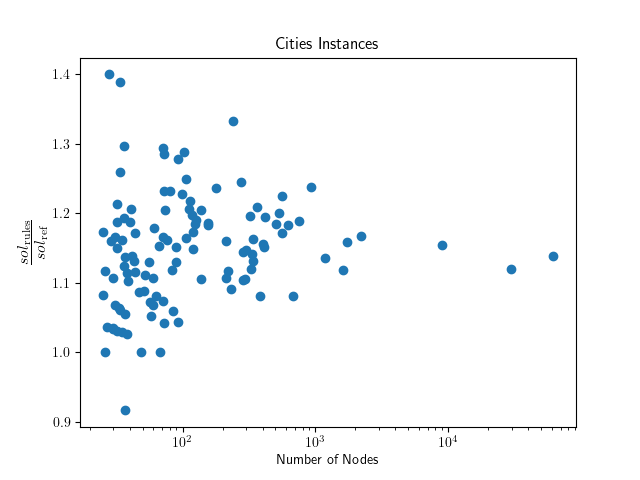
\includegraphics[width=270px]{value_rules_vs_ref}
\end{frame}

\begin{frame}{Rules-Heuristik: Laufzeit}
    \centering
    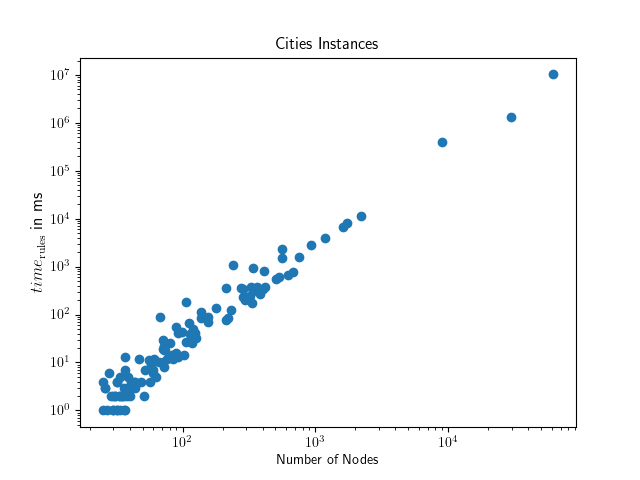
\includegraphics[width=270px]{rules_time_abs}
\end{frame}

\begin{frame}{Rules-Heuristik: Vergleich mit SAN}
    \centering
    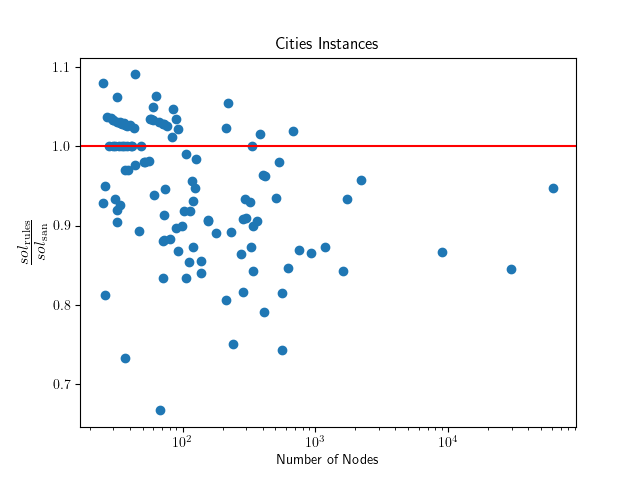
\includegraphics[width=270px]{value_rules_vs_san}
\end{frame}

\begin{frame}{Rules-Heuristik: Vergleich mit SAN: Laufzeit}
    \centering
    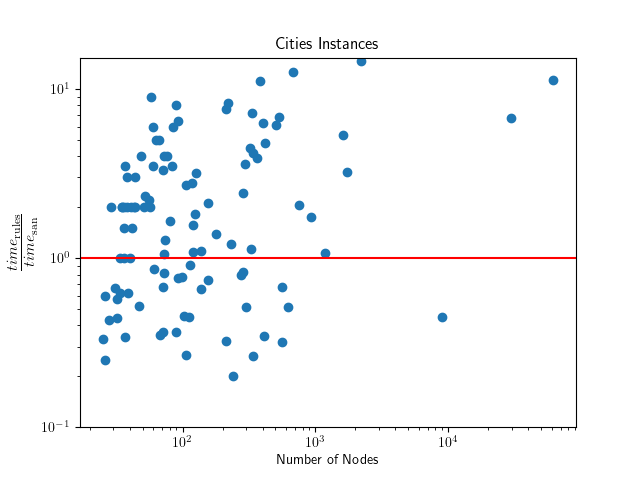
\includegraphics[width=270px]{time_rules_vs_san_1}
\end{frame}

\end{document}